\documentclass[10pt]{beamer}
% Beamer uses a standard paper size of 128x96mm

% ===== Packages =====
\usepackage[utf8]{inputenc}
\usepackage[T1]{fontenc}

\usepackage{graphicx}
\usepackage{tikz}  % TODO: utilisé pourquoi? (il est particulierement lent a compiler avec)
\usepackage{enumitem} % Custom lists

\usepackage[backend=biber, autolang=other, style=phys, sorting=none]{biblatex}  % Citing
\addbibresource{../bibliography/bibliography.bib}

% ===== Typeface =====
\usepackage{mlmodern} % thicker math, do not touch

% \usepackage[sfdefault]{FiraSans} % peculiar but nice
% \usepackage{tgheros} % nice
\usepackage[sfdefault]{plex-sans} % nice
% \usepackage[sfdefault]{noto}
% \usepackage[sfdefault, light]{FiraSans} 
% \usepackage{helvet}
% \usepackage[sfdefault]{AlegreyaSans} % peculiar
% \usepackage{montserrat}
% \usepackage{raleway}
% \usepackage{avant} % nah
% \usepackage{tgadventor} % nah
% \usepackage{cmbright} % meh
% \usepackage{DejaVuSans} % big
% https://tug.org/FontCatalogue/sansseriffonts.html

% ===== Beamer theme =====
\usetheme{Boadilla} % other interesting built-in: Boadilla, CambridgeUS (if we want sections in header), Pittsburgh (super-plain)

\setbeamertemplate{footline}{   % only page number in footline
    \hfill%
    \usebeamercolor[fg]{page number in head/foot}%
    % \usebeamerfont{page number in head/foot}%
    \small%
    \setbeamertemplate{page number in head/foot}[framenumber]%
    \usebeamertemplate*{page number in head/foot}\kern1em\vskip4pt%
    }
    \addtobeamertemplate{footline}{\vspace*{-0.5cm}}{}
    
    \setbeamertemplate{blocks}[rounded][shadow=false]
    \setbeamertemplate{navigation symbols}{}
    
% ===== Colors =====
% \usecolortheme{beaver}
\definecolor{UBCblue}{rgb}{0.04706, 0.13725, 0.26667} % UBC Blue (primary)
\usecolortheme[named=UBCblue]{structure}

% \setbeamercolor{block title}{bg=cyan!50, fg=white} % modifying colors (the ! is for trasparency)
% \definecolor{darkred}{rgb}{0.8,0,0}

% \setbeamercolor{section in toc}{fg=black,bg=white}
% \setbeamercolor{alerted text}{fg=darkred!80!gray}
% \setbeamercolor*{palette primary}{fg=darkred!60!black,bg=gray!30!white}
% \setbeamercolor*{palette secondary}{fg=darkred!70!black,bg=gray!15!white}
% \setbeamercolor*{palette tertiary}{bg=darkred!80!black,fg=gray!10!white}
% \setbeamercolor*{palette quaternary}{fg=darkred,bg=gray!5!white}

% \setbeamercolor*{sidebar}{fg=darkred,bg=gray!15!white}

% \setbeamercolor*{palette sidebar primary}{fg=darkred!10!black}
% \setbeamercolor*{palette sidebar secondary}{fg=white}
% \setbeamercolor*{palette sidebar tertiary}{fg=darkred!50!black}
% \setbeamercolor*{palette sidebar quaternary}{fg=gray!10!white}

% \setbeamercolor*{titlelike}{parent=palette primary}
% \setbeamercolor{titlelike}{parent=palette primary,fg=darkred}
% \setbeamercolor{frametitle}{bg=gray!10!white}
% \setbeamercolor{frametitle right}{bg=gray!60!white}

% \setbeamercolor*{separation line}{}
% \setbeamercolor*{fine separation line}{}

% \definecolor{cyanish}{RGB}{10,250,250}  % different ways to define colors
% \definecolor{lightgreen}{HTML}{CCFF99}
% \definecolor{orangish}{wave}{620}
% \colorlet{ochre}{blue!30!yellow!70!}

% ===== Text properties =====
\renewcommand*\familydefault{\sfdefault} % sans-serif as default
% \linespread{1.3} % Change line spacing
\usefonttheme{professionalfonts} % uses Computer Modern for math as God intended
\setbeamerfont{bibliography entry author}{size=\scriptsize, series=\normalfont} 
\setbeamerfont{bibliography entry title}{size=\scriptsize, series=\bfseries} 
\setbeamerfont{bibliography entry location}{size=\scriptsize, series=\normalfont} 

% ===== Avoid footnotes at the end of columns =====
\makeatletter
\renewrobustcmd{\blx@mkbibfootnote}[2]{%
\iftoggle{blx@footnote}
{\blx@warning{Nested notes}%
\addspace\mkbibparens{#2}}
{\unspace
\ifnum\blx@notetype=\tw@
\expandafter\@firstoftwo
\else
\expandafter\@secondoftwo
\fi
{\csuse{blx@theendnote#1}{\protecting{\blxmkbibnote{end}{#2}}}}
{\csuse{footnote#1}[frame]{\protecting{\blxmkbibnote{foot}{#2}}}}}}
\makeatother
% \setlist[itemize]{label={$\vcenter{\hbox{\scriptsize$\bullet$}}$}, leftmargin=0.6cm, topsep=-3pt}
\setlist[itemize]{label={--}, leftmargin=0.6cm}

% ===== Global background =====
% %Global Background must be put in preamble
% \usebackgroundtemplate%
% {%
%     \includegraphics[width=\paperwidth,height=\paperheight]{newton.jpg}%
% }

% ===== Title logo =====
\titlegraphic { 
\begin{tikzpicture}[overlay,remember picture]
\node[right=0.2cm] at (current page.147){
    
\includegraphics[width=1.5cm]{../figures/EPFL_logo.png}
};
\end{tikzpicture}
}
% Or more simply:
% \titlegraphic{
\includegraphics[width=1.5cm]{../figures/EPFL_logo.png}} % Title logo

% ===== Commands =====
\newcommand{\probecurrent}[0]{\ensuremath{I_{\mathrm{probe}}}}
\newcommand{\electronsaturationcurrent}[0]{\ensuremath{I_{e,{\mathrm{sat}}}}}


% ===== Presentation =====
\title[(À enlever)]{Argon plasma analysis using Langmuir probes}
\author[Tom Vadot \and Matteo Veneziano]{Tom Vadot \and Matteo Veneziano}
\institute[]{EPFL Section of Physics}
\date{November 29, 2024}
% \logo{
\includegraphics[width=1.5cm]{../figures/EPFL_logo.png}} % logo en chaque page

\begin{document}

\begin{frame}
    \titlepage
\end{frame}

\section{Introduction}
\begin{frame}{Introduction}
    intro
\end{frame}

\section{Theory and experimental setup}
\begin{frame}{Defining plasma}
    A \emph{quasineutral} gas of charged and neutral particles which exhibit \emph{collective} behaviour" \footfullcite{chen_introduction_2006}
    \vspace{0.5cm}
    \begin{itemize}
        \item \textbf{Quasineutrality}: even though the particles making up a plasma consist of free electrons and ions, their overall charge densities cancel each other in equilibrium: 
            $n_e \simeq Z n_i$ \footfullcite{gibbon_introduction_2016}

        \item \textbf{Collective behaviour}: macroscopic fields dominate over short-lived microscopic fluctuations.
            An external stimulus creates a simultaneous response of many particles \footfullcite{piel_plasma_2017}.
    \end{itemize}
    \vspace{0.5cm}
    Cold plasma: ions are not thermalised and electrons have a temperature such that $T_e \gg T_i$ \footfullcite{bagnato_notice_2019}.
\end{frame}


\begin{frame}{Langmuir probes}
    Widely used devices for measuring different properties of plasma, e.g. electron temperature and density.
    \vspace{0.4cm}

    They consist of a plane electrode OF SURFACE A PROBE (e.g. a small tantalum disk) inserted into the chamber and biased by an external voltage.
    The charges (both ions and electrons) reach the surface and generate probe current $\probecurrent$, which is measured\footfullcite{piel_plasma_2017}.
    NOTE: DONNER FORMULE RELATION ENTRE BIAIS, PLASMA, PROBE ET LA FORMULE DU COURANT
    \centering
    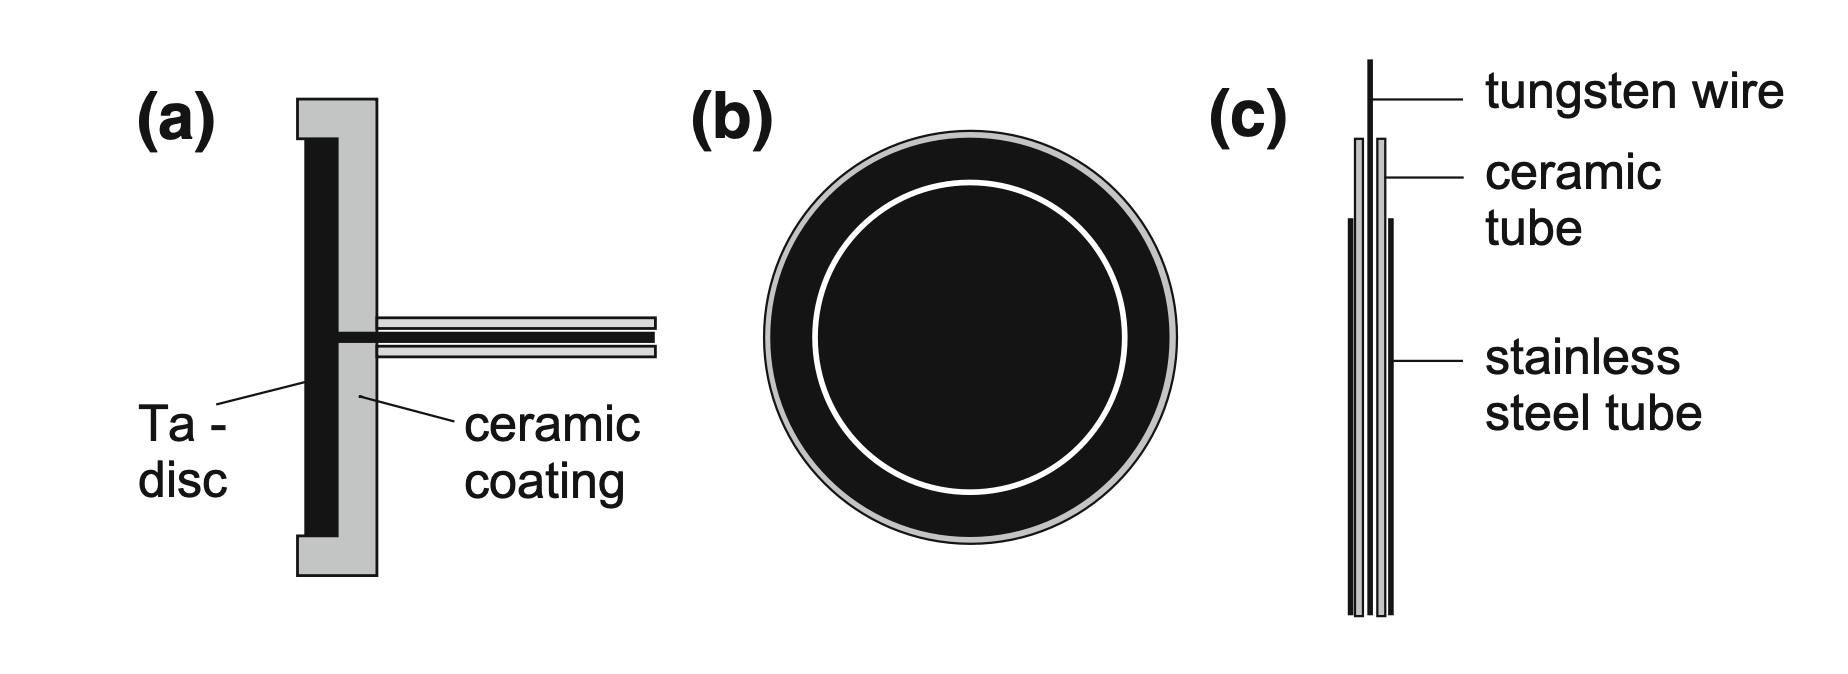
\includegraphics[width=0.75\textwidth]{../figures/langmuir_probe.png}
\end{frame}


\begin{frame}{The $I$--$V$ characteristic curve}
    Measure of the probe current as a function of the bias potential.
    Three regions
    \begin{enumerate}
        \item[I] High negative bias: no electrons reach the probe. Constant ion saturation current.
        \item[II] Electron retardation regime: part of the electrons reach the probe. The electron current increases exponentially with the bias voltage (\footfullcite{piel_plasma_2017} or \footfullcite{bagnato_notice_2019})
            \begin{equation*}
                I = blabla
            \end{equation*}
        \item[III] High positive bias: constant electron saturation current.
    \end{enumerate}
    Two points of physical significance
    \begin{itemize}
        \item Floating potential $\Phi_f$: no current flows in the probe
        \item Plasma potential $\Phi_p$: the potential inside the ambient plasma, corresponds to electron saturation current
            \begin{equation*}
                \electronsaturationcurrent = \frac{1}{4}e n_e v_{e,th} A_{\mathrm{probe}}
            \end{equation*}
    \end{itemize}
\end{frame}

\begin{frame}{Extracting electron temperature and density}

\end{frame}


\begin{frame}{Ion acustic waves}
    
\end{frame}


\begin{frame}{Experimental setup}
    Prendre figure dans vieux rapport et citer.
    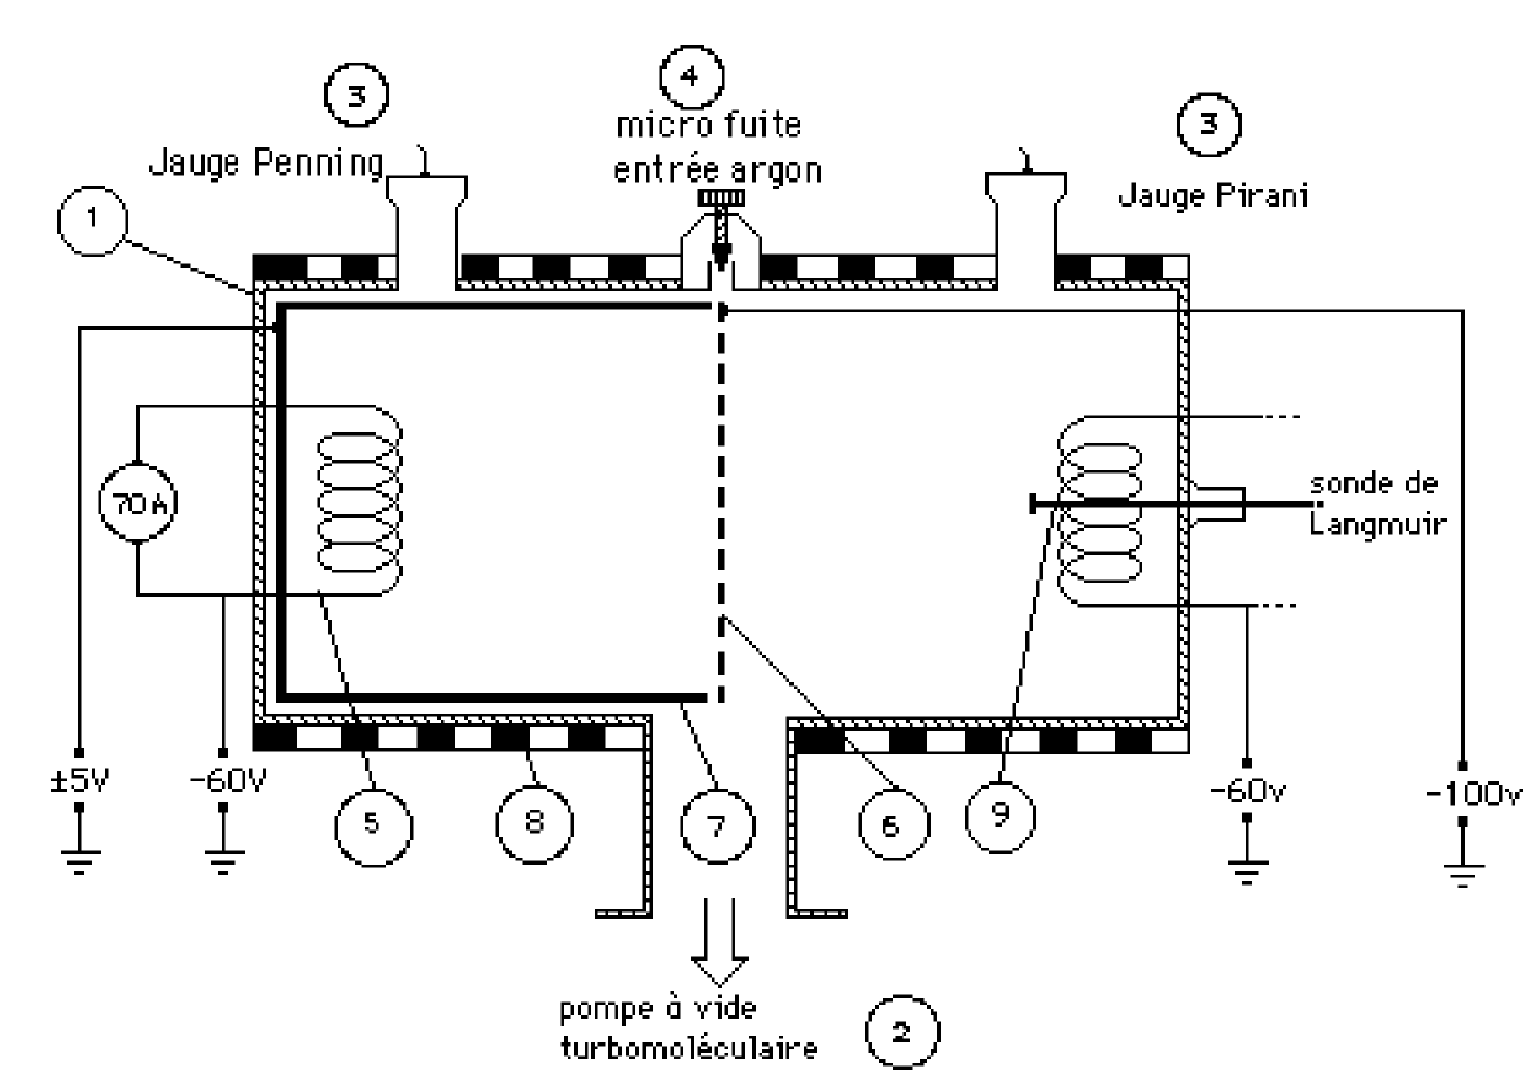
\includegraphics[width=6cm]{../figures/experimental-setup.png}
\end{frame}

\section{Results}
\begin{frame}{(Variation avec position, differentes pressions)}{Legend outside!}
    \begin{columns}[T]
        \column{0.5\textwidth}
        \centering
        \begin{figure}
            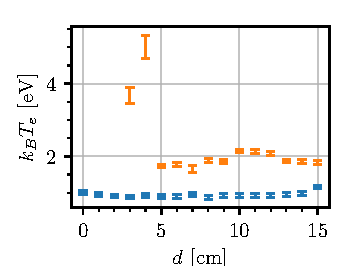
\includegraphics[scale=1]{../figures/temperatureeV_position.pdf}
            \caption{ciao}
        \end{figure}

        \column{0.5\textwidth}
        \centering
        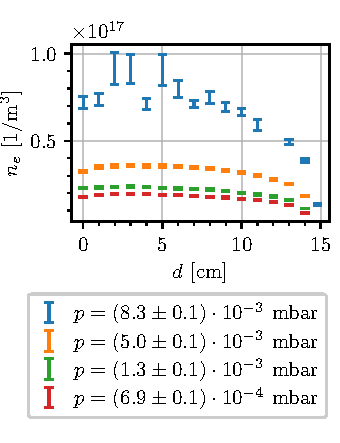
\includegraphics[scale=1]{../figures/density_position.pdf}
    \end{columns}

    \begin{itemize}
            \item Close to heating elements \(\rightarrow\) higher \(e^-\) temperature
            \item Higher pressure decreases temperature
            \item Maximal density for distances 3-6 cm from heating element (or is it completely arbitrary?)
    \end{itemize}
\end{frame}
    
\begin{frame}{Variation avec pression}{IMPORTANT! donner les autres parametres (ceux qui n'ont pas été variés pour faire le plot)}
    "Ensuite on a mieux etudié la variation en pression"
    \begin{columns}
        \column{0.5\textwidth}
        \centering
        \fbox{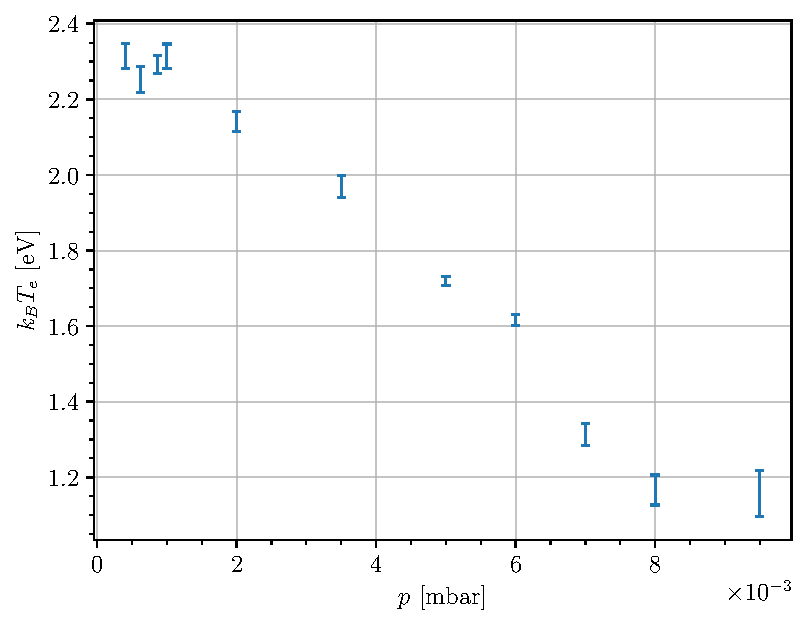
\includegraphics[scale=1]{../figures/temperatureeV_pressure.pdf}}

        As observed before, higher pressure decreases temperature.

        \column{0.5\textwidth}
        \centering
        \fbox{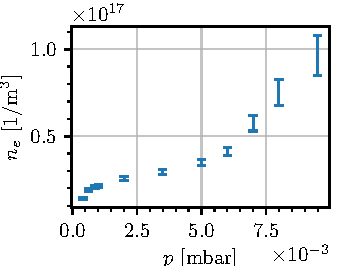
\includegraphics[scale=1]{../figures/density_pressure.pdf}}
        Higher pressure leads to higher density.

    \end{columns}
\end{frame}

\begin{frame}{Variation avec filament current}{IMPORTANT! donner les autres parametres (ceux qui n'ont pas été variés pour faire le plot)}
    \begin{columns}
        \column{0.5\textwidth}
        \centering
        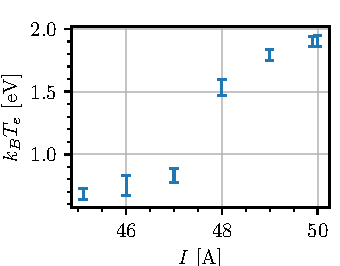
\includegraphics[scale=1]{../figures/temperatureeV_current.pdf}


        \column{0.5\textwidth}
        \centering
        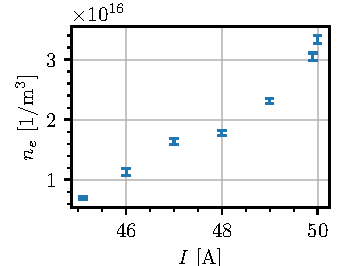
\includegraphics[scale=1]{../figures/density_current.pdf}

    \end{columns}
\end{frame}

\begin{frame}{Variation avec filament polarisation}{IMPORTANT! donner les autres parametres (ceux qui n'ont pas été variés pour faire le plot)}
    \begin{columns}
        \column{0.5\textwidth}
        \centering
        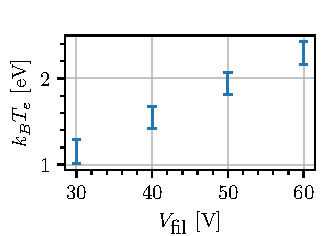
\includegraphics[scale=1]{../figures/temperatureeV_filament_polarisation.pdf}


        \column{0.5\textwidth}
        \centering
        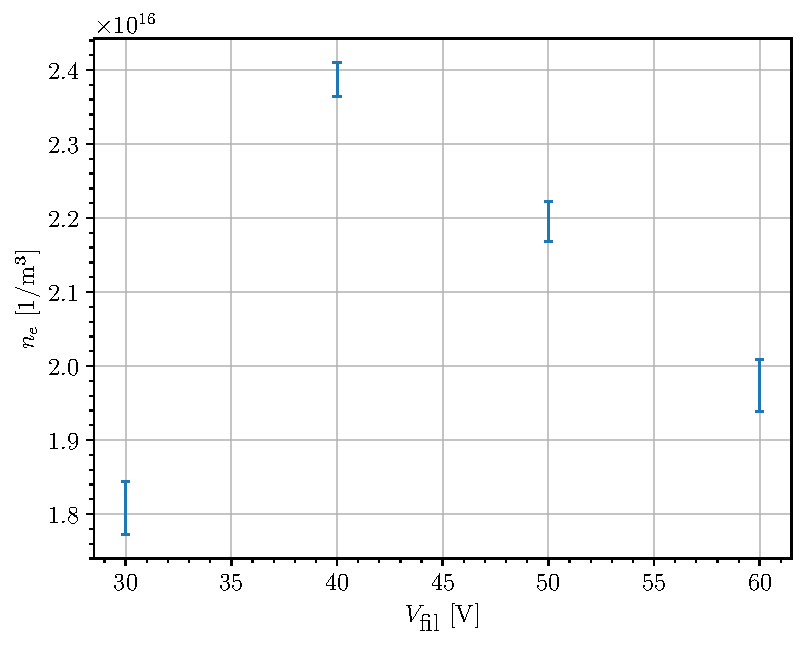
\includegraphics[scale=1]{../figures/density_filament_polarisation.pdf}

    \end{columns}
\end{frame}

\begin{frame}{Variation avec position radiale}
    \begin{columns}
        \column{0.5\textwidth}
        \centering
        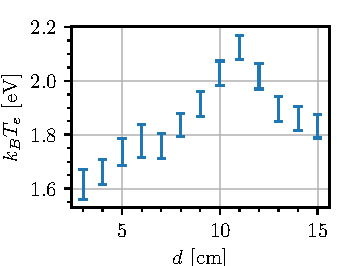
\includegraphics[scale=1]{../figures/temperatureeV_position_radial.pdf}

        \column{0.5\textwidth}
        \centering
        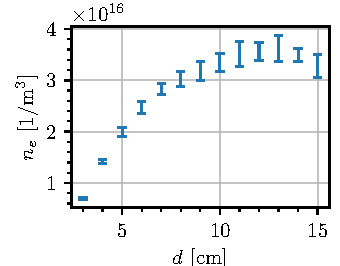
\includegraphics[scale=1]{../figures/density_position_radial.pdf}

    \end{columns}
\end{frame}

\begin{frame}{Difference between using one and two filaments}
    {A study in position}
    Until here, only one filament was used to do the thing.
    \begin{columns}
        \column{0.5\textwidth}
        \centering
        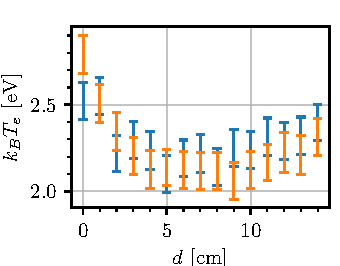
\includegraphics[scale=1]{../figures/temperatureeV_position_twofilaments.pdf}

        \column{0.5\textwidth}
        \centering
        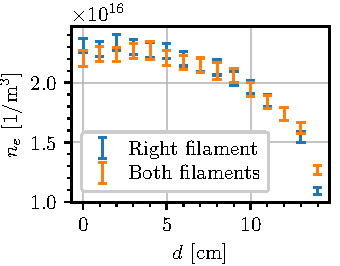
\includegraphics[scale=1]{../figures/density_position_twofilaments.pdf}

    \end{columns}
\end{frame}

\section{Discussion}
\begin{frame}{Hysteresis}
    During measures,
    hysteresis observed for high current and (high?) pressure, caused by impurities\footfullcite{hassouba_analysis_2013}
    \begin{center}
        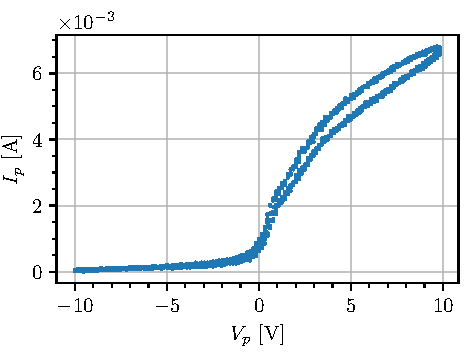
\includegraphics[scale=1]{../figures/hysteresis.pdf}
    \end{center}

\end{frame}


% \begin{frame}{Some other stuff about Plasma}{Now with lines!}
%     \begin{columns}
%     % Column 1
%     \begin{column}{0.49\textwidth}
%         \begin{itemize}
%             \item Mmmh yes the plasma is made of plasma
%             \item It do be warm tho (and cold too how cool is that?)
%             \item Third smart remark
%         \end{itemize}
%     \end{column}
%    % Column 2 (vertical line)
%     \begin{column}{.02\textwidth}
%         \rule{.1mm}{0.7\textheight}
%     \end{column}
%    % Column 3    
%     \begin{column}{0.49\textwidth}
%         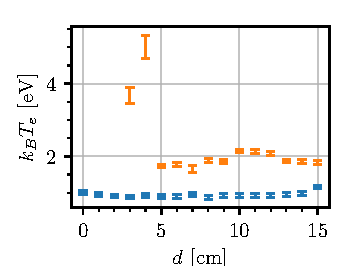
\includegraphics[width=\textwidth]{../figures/temperatureeV_position.pdf}
%     \end{column}
%     \end{columns}
% \end{frame}



% \begin{frame}{Overlays in Beamer}
%     The easiest way is to use the stop command
%     \pause

%     Like this
%     \pause

%     There are other very customisable ways but we won't need them.
%     \pause

%     wait i can animate anything here
%     \pause

%     you just lost the game
% \end{frame}

\end{document}